
\section{B1}

\subsection{B1.1}

\subsubsection{a + b}

See appendix B1.1, a+b.

There is a current queue index,
which is selected according to the number
of tickets of each task every time the time quota
has run out.

\subsubsection{c}

\begin{verbatim}
P=? [F<=time finished]
\end{verbatim}

\begin{figure}[!htb]
\centering
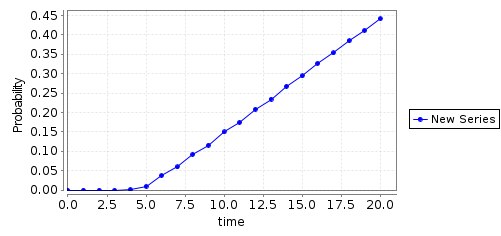
\includegraphics[scale=.75]{images/B1_1_c.png}
\caption{Probability for client finishing its first task within 0 to 20 timesteps}
\label{fig:nojobprop}
\end{figure}

\subsubsection{d}

No, because a job in the queue always has at least one ticket,
and as long as it has one ticket, it cannot perpetually be
be stuck in the queue.

\subsubsection{e}

See appendix B1.1, e.

\begin{figure}[!htb]
\centering
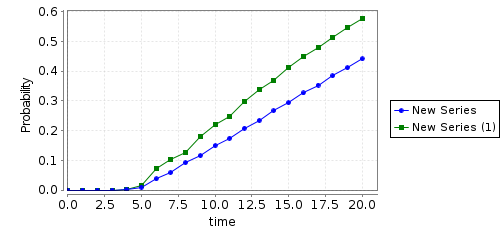
\includegraphics[scale=.75]{images/B1_1_e.png}
\caption{Probabilities for client finishing its first task within 0 to 20 timesteps.
Second series is with time quota equal 2}
\label{fig:nojobprop}
\end{figure}

It seemingly makes the probability higher earlier,
but this may be due to the diminished overhead
from selecting the next job to perform,
since it takes one step to select it.

\subsection{B1.2}

\subsubsection{a}

See appendix B1.2, a.

There are different ways to approximate an SRT-scheduler.
If the approximation ensures that a job in the queue always
has at least one ticket, there can be no starvation.

The chosen scheduling is giving a client a number of tickets
equal to 6 - task*.
This way, tasks with short length, such as 1 or 2,
get many tickets, while tasks with long length such as 5,
get few (but still a positive number of) tickets.

It should be noted that a time quota of 1 is used.

\subsubsection{b}

\begin{figure}[!htb]
\centering
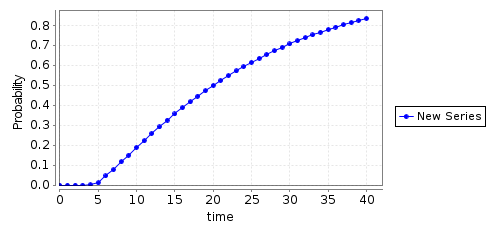
\includegraphics[scale=.75]{images/B1_2_a.png}
\caption{Probabilitiy for client finishing its first task within 0 to 40 timesteps, SRT.}
\label{fig:nojobprop}
\end{figure}

Makes the probability a bit higher than the previous with time quota 1.

\subsubsection{c}

The maximum was 4 clients.

\subsubsection{d}

See appendix B1.2, d.

\begin{figure}[!htb]
\centering
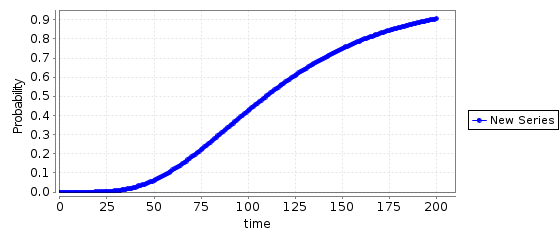
\includegraphics[scale=.75]{images/B1_2_d.png}
\caption{Probabilitiy for client finishing its first task within 0 to 200 timesteps, SRT, fast and slow-job combination.}
\label{fig:nojobprop}
\end{figure}

We let client 1, 3 and 4 produce jobs of length 1, and client 2 produce jobs of length 5.

The probability of finishing rises much, much more slowly over time,
but since the jobs from client 2 still have a ticket, they will never
be completely starved.
While it will take much longer for it to get finished, it will almost certainly (ie. with probability 1.0)
be finished at some point.

\subsubsection{e}

If denial of service is understood as starvation,
then we can say that whenever a job is in the queue for client 2,
it will almost certainly get out of the queue at some point.

\begin{verbatim}
P>=1 [G (state2=1 => P>=1 [F state2=0])]
\end{verbatim}

PRISM verifies it as holding.

